\section{Desenvolvimento}

\subsection{Questão 1}
\textbf{Qual a função de transferência contínua do sistema para os valores numéricos do seu grupo? Quais os pólos do sistema de segunda ordem contínuo? Qual a classificação do sistema de segunda ordem (sobreamortecido, criticamente amortecido ou subamortecido)? Para obter os pólos da função de transferência, o seguinte comando de Matlab pode ser utilizado considerando que a função de transferência \( G \) já foi definida:}
\begin{verbatim}
p = pole(G)
\end{verbatim}

A função de transferência \( G(s) \) é obtida pelo Matlab:

\begin{verbatim}
    zeta = 1.012
    wn = 0.875
    R = 1.18;
    g = tf(wn^2, [1 2*zeta*wn wn^2]) % Funcao de Transferencia
\end{verbatim}

Tal que a função de transferência para os valores númericos do meu grupo pode ser observada na Equação \ref{eq:G(s)_numerico}
\begin{equation}
\label{eq:G(s)_numerico}
   G(s) = \frac{0.765625}{s^2 + 1.7755s + 0.765625}
\end{equation}

   Para encontrar os pólos do sistema, resolvemos a equação característica dada pelo denominador da função de transferência:

   \[
   s^2 + 1.7755s + 0.765625 = 0
   \]

   Assim, os pólos são:

   \[
   s_1 = \frac{-1.7755 + 0.3081}{2} = -0.7337
   \]

   \[
   s_2 = \frac{-1.7755 - 0.3081}{2} = -1.0418
   \]

   Portanto, os pólos do sistema são aproximadamente \( s_1 = -0.7337 \) e \( s_2 = -1.0418 \).

   A classificação do sistema pode ser feita a partir do coeficiente de amortecimento \( \zeta \):

\begin{itemize}
    \item \textbf{Sobreamortecido:} \( \zeta > 1 \)
    \item \textbf{Criticamente Amortecido:} \( \zeta = 1 \)
    \item \textbf{Subamortecido:} \( \zeta < 1 \)
\end{itemize}

   Com \( \zeta = 1.012 \), o sistema é \textbf{sobreamortecido}, pois o coeficiente de amortecimento é maior que 1.

\vspace{10pt}
\hrule

\subsection{Questão 2}
\textbf{Mostre no relatório qual o período de amostragem escolhido baseado na largura de banda do sistema. Como você chegou no valor para o período de amostragem? Mostre no relatório a largura de banda em [rad/s] e em [Hz], e também a frequência de amostragem em [rad/s] e em [Hz]. Observação: o valor escolhido para \( T_0 \) baseado na largura de banda deve ser maior que 0,2 segundos. Justifique se precisar usar um valor igual ou menor.}

Como vimos na Prática 2, a frequência de Nyquist exige que nossa frequência de amostragem seja pelo menos duas vezes maior que a nossa frequência de banda, todavia no mundo real isso não nos dá margem de variação, por isso, o ideal \textcolor{red}{\textbf{ADICIONAR REFERENCIA}} é que nossa frequência de amostragem seja pelo menos dez vezes maior. Desse modo, chegamos em um período de amostragem igual a $1,137s$.

\begin{verbatim}
    wb = bandwidth(g)
    fb = wb/(2*pi)
    F0 = 10*fb
    W0 = F0*2*pi
    T0 = 1/F0
\end{verbatim}

Os resultados encontrados podem ser observados na Tabela \ref{tab:wb-fb-F0-W0}

\begin{table}[H]
    \centering
    \begin{tabular}{|c|c|c|} \hline 
         &Largura de Banda&  Frequência de Amostragem\\ \hline  
         Hertz&  $0.0879$&  $0.8795$\\ \hline  
         Rad/s&  $0.5526$ &  $5.5259$\\ \hline 
    \end{tabular}
    \caption{Largura de banda e frequência de amostragem}
    \label{tab:wb-fb-F0-W0}
\end{table}

\vspace{10pt}
\hrule

\subsection{Questão 3}
\textbf{A partir da função de transferência contínua do sistema, encontre e mostre no relatório a função de transferência discreta do sistema considerando um retentor de ordem zero. Para isso, considerando que a função de transferência contínua já foi definida no Matlab como sendo \( G \), e o período de amostragem foi definido como sendo \( T_0 \), utilize o seguinte comando no Matlab:}
\begin{verbatim}
Gz = c2d(G, T0, 'zoh')
\end{verbatim}

A função de transferência discreta do sistema \texttt{Gz} é dada pela Equação \ref{eq:Gz_discreto}.

\begin{equation}
\label{eq:Gz_discreto}
   G(s) = \frac{0.2609 z + 0.1331}{z^2 - 0.7395z + 0.1335}
\end{equation}

\vspace{10pt}
\hrule

\subsection{Questão 4}
\textbf{Quais os pólos e zeros da função de transferência discreta? Para obter os zeros da função de transferência, o seguinte comando de Matlab pode ser utilizado considerando que a função de transferência \( Gz \) já foi definida:}
\begin{verbatim}
z = zero(Gz)
\end{verbatim}

Os pólos podem ser obtidos utilizando o seguinte comando no Matlab:

\begin{verbatim}
p = pole(Gz)
\end{verbatim}

Os resultados obtidos foram:

\[
z = -0.5101
\]

\[
p_1 = 0.4265, \quad p_2 = 0.3130
\]

Portanto, a função de transferência discreta apresenta um zero em \( z = -0.5101 \) e dois pólos em \( p_1 = 0.4265 \) e \( p_2 = 0.3130 \).

\vspace{10pt}
\hrule

\subsection{Questão 5}
\textbf{Plote a resposta do sistema contínuo a uma entrada degrau de amplitude \( r \), indicada na tabela de parâmetros fornecida. Sobreponha a resposta contínua à resposta discreta. Utilize a seguinte sequência de comandos do Matlab considerando que a função de transferência contínua \( G \), a função de transferência discreta \( Gz \), e a amplitude do degrau \( r \) já foram definidas:}
\begin{verbatim}
figure
step(r*G)
hold on
step(r*Gz)
\end{verbatim}
\textbf{Acrescente título e legenda para completar a figura.}

A resposta do sistema contínua a uma entrada degrau de amplitude \(r\) pode ser observada na Figura \ref{fig:contOVERdisc}

\begin{figure}[H]
    \centering
    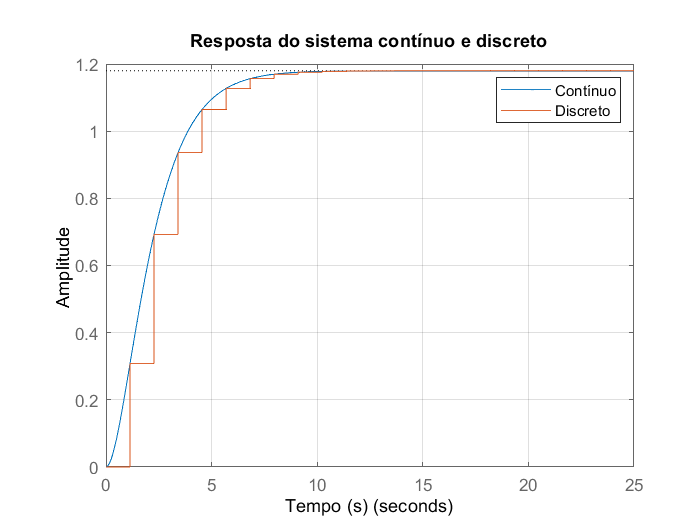
\includegraphics[width=0.6\linewidth]{pratica3/imagens/continousOVERdiscreete.png}
    \caption{Função de transferência contínua e função de transferência discreta}
    \label{fig:contOVERdisc}
\end{figure}

\vspace{10pt}
\hrule

\subsection{Questão 6}
\textbf{Qual o tempo de acomodação (\( t_s \)) da resposta do sistema discreto considerando o critério de ±2\%? Qual o tempo de subida (\( t_r \)) da resposta do sistema discreto? Para encontrar esse valor, clique com o botão direito do mouse no gráfico mostrado pelo Matlab como resposta ao comando \texttt{step}. Então selecione \textit{Characteristics}, e depois \textit{Settling Time} (\( t_s \)) e \textit{Rise Time} (\( t_r \)).}

O tempo de acomodação do sistema é de $6,82s$ e o de subida $4,09s$. Os resultados podem ser observados na Figura \ref{fig:rise-settling-time}

\begin{figure}[H]
    \centering
    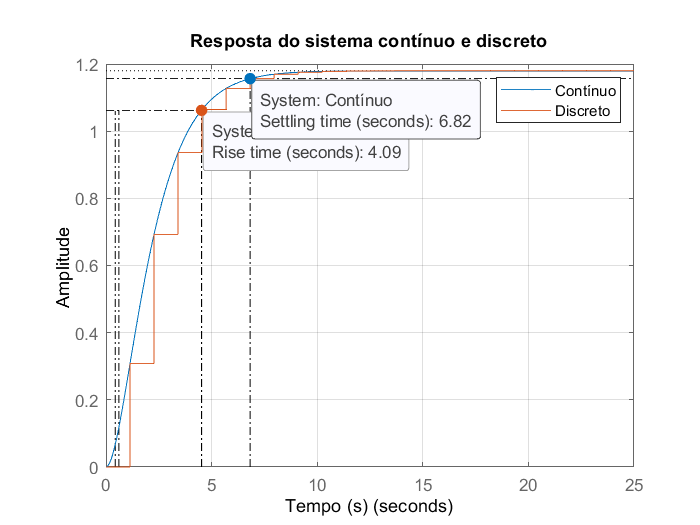
\includegraphics[width=0.6\linewidth]{pratica3/imagens/riseANDsettlingTIME.png}
    \caption{Tempo de acomodação e tempo de subida do sistema discreto}
    \label{fig:rise-settling-time}
\end{figure}
\vspace{10pt}
\hrule

\subsection{Questão 7}
\textbf{Utilizando o Simulink, implemente o diagrama da Figura \ref{fig:simulink-goal} que faz a simulação do sistema contínuo em malha aberta submetido a uma entrada degrau. Sequência a ser utilizada para isso:}
\begin{enumerate}
    \item \textbf{Abra o Simulink digitando \texttt{simulink} no prompt da janela de comando do Matlab, ou utilize o botão disponível na aba \textit{Home}.}
    \item \textbf{Quando a janela do Simulink abrir, escolha a opção de criar um \textit{Blank Model}.}
    \item \textbf{Clique no botão \textit{Library Browser}.}
    \item \textbf{Arraste do \textit{Library Browser} para a área em branco à direita os blocos que você vai utilizar para criar o diagrama (Transfer Fcn, Zero-Order Hold, Scope, To Workspace, Step). Eles podem ser encontrados dentro da categoria \textit{Simulink} nas sub-categorias: \textit{Continuous}, \textit{Discrete}, \textit{Sinks}, \textit{Sources}.}
    \item \textbf{Conecte os blocos clicando na entrada de um bloco e arrastando para a saída de outro bloco ou ponto de conexão desejado.}
    \item \textbf{Configure o tempo de simulação para 15 segundos alterando o valor de \textit{Stop Time} na barra superior da janela do Simulink.}
    \item \textbf{Configure as propriedades de cada bloco:}
    \begin{itemize}
        \item \textbf{\textit{Step}: Ajustar o \textit{Step Time} para 0, ajustar o \textit{Final Value} para o valor da amplitude do degrau \( r \);}
        \item \textbf{\textit{Transfer Function}: Insira os vetores com os valores dos coeficientes do polinômio do numerador e denominador da função de transferência (ordem decrescente de expoentes). Para recuperar os vetores que representam os polinômios do numerador e denominador da função de transferência:
        \texttt{[num, den] = tfdata(G, 'v')}
        }
        \item \textbf{\textit{Zero-Order Holder}: Configure o \textit{Sample Time} como sendo o valor do período de amostragem \( T_0 \) escolhido;}
        \item \textbf{\textit{To Workspace}: Configure o \textit{Variable name} para o nome da variável do workspace onde você quer armazenar os dados. Por exemplo, \texttt{yc} para a saída contínua, e \texttt{yd} para a saída discreta.}
    \end{itemize}
    \item \textbf{Execute a simulação apertando o botão de play da barra superior da janela do Simulink.}
\end{enumerate}

\begin{figure}[H]
    \centering
    \includegraphics[width=0.75\linewidth]{pratica3//imagens/diagrama-simulink.png}
    \caption{Diagrama do Simulink a ser implementado}
    \label{fig:simulink-goal}
\end{figure}

A implementação feita no Simulink pode ser observada na Figura \ref{fig:simulink-done}.

\begin{figure}[H]
    \centering
    \includegraphics[width=0.75\linewidth]{pratica3//imagens/simulink-done.png}
    \caption{Simulink implementado pelos autores}
    \label{fig:simulink-done}
\end{figure}

\vspace{10pt}
\hrule

\subsection{Questão 8}
\textbf{Mostre no relatório uma figura com as saídas sobrepostas geradas pelo Simulink e exportadas pelos blocos \textit{To Workspace}. Para plotar os dados exportados pelos blocos \textit{To Workspace} utilize a seguinte sequência de comandos no Matlab:}
\begin{verbatim}
figure
plot(out.yc.Time, out.yc.Data, 'b')
hold on
stairs(out.yd.Time, out.yd.Data, 'r')
\end{verbatim}
\textbf{Acrescente título e legenda para completar a figura. Observe que a saída discreta obtida utilizando o retentor de ordem zero no Simulink é a mesma saída obtida pelo comando \texttt{step} aplicado na função de transferência discreta.}

As saídas geradas pelo Simulink podem ser observadas na Figura \ref{fig:simulink-continous-discreete}

\begin{figure}[H]
    \centering
    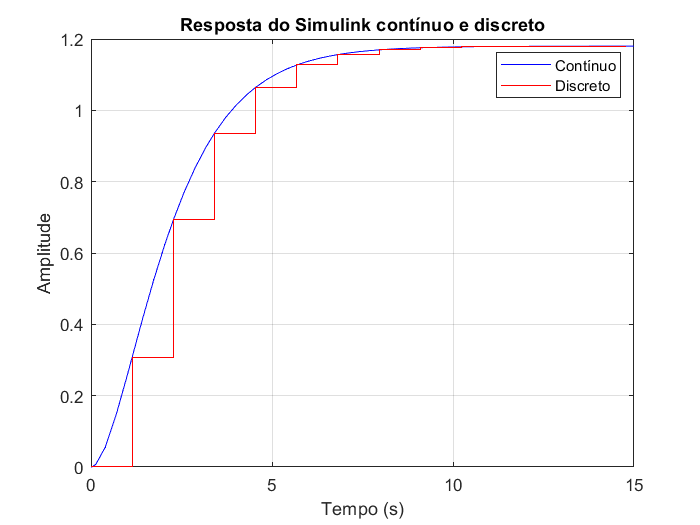
\includegraphics[width=0.75\linewidth]{pratica3/imagens/simulink-continouosOVERdiscreete.png}
    \caption{Saída gerada pelos blocos Simulink}
    \label{fig:simulink-continous-discreete}
\end{figure}

\vspace{10pt}
\hrule
